\chapter{Contexte Général du projet}

Ce chapitre représente une mise en contexte du projet en se focalisant dans la première partie sur son cadre à travers la présentation de la problèmatique qu'il doit résoudre. La deuxième partie aura comme but d'éclaircir l'objectif général à atteindre ainsi les différentes exigences à respecter avant d'attaquer dans la dernière partie, l'organisation méthodologique mise en œuvre pour réaliser ce projet.

\section{Présentation générale du projet}

Au royaume de la santé digitale, l'application pour smartphone est reine. Selon Proxima Mobile, le portail de services aux citoyens sur terminaux mobiles, on comptait $6 000$ applications mobiles médicales en $2010$, près de $20 000$ en $2012$, près de $100 000$ aujourd'hui. Selon le cabinet research2guidance, le marché des services de santé mobile pourrait atteindre $26$ milliards de dollars au niveau mondial d'ici $2017$... Diabète, allergies, sida, guide santé pour les voyageurs, sevrage tabagique... Les applications santé à destination des patients sont nombreuses, dont certaines sont conçues pour les professionnels de santé $[W1]$.

\vspace{6pt}
\paragraphmark

Avec l'explosion des applications de suivi personnel (permettant à leurs utilisateurs de contrôler en direct leur temps de marche, calories dépensées, temps de sommeil, mesurer la pression sanguine...), la e-santé prend une part de plus en plus importante dans notre société.

\subsection{Problèmatique}

Le développement des nouvelles technologies de l’information et de la communication dans les domaines sanitaire et médico-social ainsi que des modes d’exercice pluridisciplinaire accroissent le besoin d’échange dans l’intérêt d’une meilleure prise en charge des personnes. Les données de santé et les données médico-sociales sont aujourd’hui des données destinées à être partagées, même si elles relèvent de la vie privée de la personne $[W2]$.

\vspace{6pt}
\paragraphmark

Comment alors permettre un tel échange de données de santé tout en protégeant la vie privée des patients? 

\subsection{Objectifs du projet}

L'objectif principal du projet est de développer une application mobile de santé préservant la vie privée des patients en applicant l'approche PPAMH. Cet objectif global se décline en plusieurs objectifs spécifiques, notamment:

\vspace{6pt}
\paragraphmark

\begin{itemize}
	\item Offrir un mécanisme d'authentification pour protéger l'accès à l'application. Il peut être basé sur un login et un mot de passe ou sur une connexion à travers les réseaux sociaux (Facebook, Google+, ..etc) afin de faciliter au maximum ce mécanisme aux différents types de patients.
	\item Permettre aux patients d'exprimer leurs préférences en ce qui concerne la divulgation de leurs renseignements personnels à l'aide d'un questionnaire afin de déterminer le degré de protection à mettre en place.
	\item Obliger les tiers (les fournisseurs Cloud et les institutions) à respecter les préférences des patients.
\end{itemize}

\vspace{6pt}
\paragraphmark

Pour atteindre nos objectifs, l'application à développer doit répondre à un certain nombre d'exigences.

\subsection{Exigences pour un système e-santé}

Les exigences nécessaires pour un système e-santé respectueux de la vie privée sont:

\subsubsection{Exigences de sécurité et de protection de la vie privée}

\begin{itemize}
	\item Exigences de sécurité: La personne (ou le groupe de personnes) désirant accéder à un dossier médical doit fournir les droits appropriés à la lecture ou à l’écriture de ce document. Le nom de la (ou les) personne(s) doit ensuite être notés dans le fichier afin de pouvoir vérifier à tout moment l’historique des accès $[1]$.

  \item Minimisation des données médicales: Un médecin peut accéder pleinement aux informations médicales de ses patients alors qu’une infirmière aura uniquement accès aux ordonnances. Dans les deux cas, et par le principe de minimisation des données, ils n’ont pas besoin de connaître les informations administratives du patient, à l’exception de son âge. Une politique d’accès précise est également utilisée pour la minimisation des données. Ce principe prévoit également l’anonymat des données médicales et donc le principe de non-associabilité des données $[1]$.

	\item Souveraineté des données: L’ensemble des informations médicales appartiennent au patient et donc ni au médecin qui les crée ou à l’hôpital qui les stocke. Cela signifie que les patients ont le contrôle de leurs données et peuvent y accéder librement. Cependant, la relation de confiance entre
un médecin et son patient donne implicitement au docteur l’accord du malade pour accéder à son dossier médical. De même, le transfert entre deux établissements doit être réalisé avec le consentement du patient $[1]$.
\end{itemize}

\subsubsection{Exigences fonctionnelles}

À travers les différents modules, l'application offrira les fonctionnalités suivantes :

\vspace{6pt}
\paragraphmark

\begin{itemize}
	\item Authentification : Le patient doit s’authentifier pour accéder à l'application. L’authentification se fera à l’aide d’un login et un mot de passe ou via une connexion à travers les réseaux sociaux (Facebook, Google+, ..etc).
	\item Questionnaire : composé de trois questions et qui permettra de déterminer les préférences du patient et par conséquent la politique de sécurité à mettre en place pour protéger sa vie privée.
	\item Base de réponses : Le patient peut consulter les réponses des médecins aux plusieurs questions fréquentes afin d'éclaircir et d'enrichir ses informations.
\end{itemize}

\subsubsection{Exigences non fonctionnelles}

Pour assurer l’efficacité de l'application, il faut respecter les critères de qualité suivants :

\vspace{6pt}
\paragraphmark

\begin{itemize}
	\item Ergonomie sobre et efficace : La mise en page du design doit faciliter au maximum la démarche de la navigation à l’aide d’une présentation claire et intuitive.
	\item Interface graphique : Les différentes couleurs et choix typographiques doivent permettrent à un patient de repérer facilement les différentes fonctionnalités qui s’offrent à lui.
	\item Espace simple: Le patient ne doit pas fournir un grand effort lors de la consultation, la mise à jour ou la sollicitation d’un service ou de son profil.
	\item Contraintes de performances : Il s’agit d’optimiser les échanges et d’utiliser des ressources de taille raisonnable afin d’avoir un temps de réponse minimal.
\end{itemize}

\subsection{Conduite du projet et planification}

Tout projet informatique requiert un cycle de développement bien défini pour assurer son succès. L’adéquation du processus de développement peut largement affecter le sort d’un projet informatique. En revanche, un mauvais choix peut conduire un projet à l’échec.

\subsubsection{Les méthodes agiles}

Les méthodes de développement dites « méthodes agiles », notées AG\footnote{AG : Agile Modeling.} visent à réduire le cycle de vie du logiciel (donc accélérer son développement) en développant une version minimale, puis en intégrant les fonctionnalités par un processus itératif basé sur une écoute
client et des tests tout au long du cycle de développement $[W3]$.

\vspace{6pt}
\paragraphmark

L’origine des méthodes agiles est liée à l’instabilité de l’environnement technologique et au fait que le client est souvent dans l’incapacité de définir ses besoins de manière exhaustive dès le début du projet. Le terme « agile » fait ainsi référence à la capacité d’adaptation aux changements de contexte et aux modifications de spécifications intervenant pendant le processus de développement.

\vspace{6pt}
\paragraphmark

Le choix de la méthode agile pour notre projet est tombé sur la méthode XP\footnote{XP : eXtreme Programming. C'est une méthode inventée par Kent Beck, Ward Cunningham et Ron Jeffries et officialisée en octobre 1999 $[W4]$.} pour le développement POO\footnote{POO : Programmation Orientée Objet.}.

\subsubsection{La méthode XP}

Extreme Programming (XP) est une méthode agile plus particulièrement orientée sur l'aspect réalisation d'une application, sans pour autant négliger l'aspect gestion de projet. Elle est adapté aux équipes réduites avec des besoins changeants $[W4]$.

\vspace{6pt}
\paragraphmark

La méthode XP couvre une grande partie des activités de la réalisation d’un logiciel $[W4]$:

\vspace{6pt}
\paragraphmark

\begin{itemize}
	\item Planification;
	\item Organisation de l’équipe de développement;
	\item Echanges avec le client;
	\item Programmation.
\end{itemize}

\vspace{6pt}
\paragraphmark

XP s'attache à rendre le projet plus flexible et ouvert au changement en introduisant des valeurs de base, des principes et des pratiques ce qui prouve un tel choix pour ce projet.

\subsubsection{La planification du projet}

La planification est parmi les phases d’avant-projet. Elle consiste à prévoir le déroulement du projet au long des phases constituant le cycle de développement.

\vspace{6pt}
\paragraphmark

Pour notre projet, nous avons utilisé le diagramme de Gantt\footnote{Diagramme de Gantt : est un outil de planification des tâches, inventé en 1910 par Henry Laurence Gantt.} afin de modéliser la planification de tâches nécessaires à la réalisation de l'application mobile Health+.

\begin{figure}[!ht]
\begin{center}
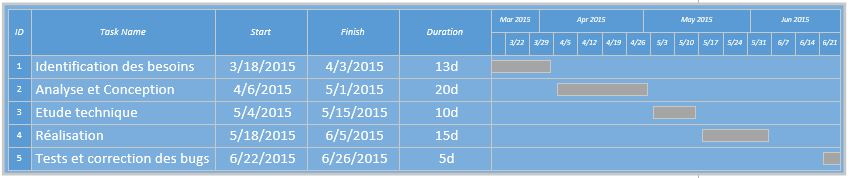
\includegraphics[scale=0.75]{gantt.JPG}
\caption{Diagramme de Gantt}
\label{gantt}
\end{center}
\end{figure}

Pour réaliser l'application, le projet est divisé en cinq tâches comme indiqué par le diagramme de gantt (figure \ref{gantt}) ci-dessus. Notons que les dates mentionnées sont sous la forme de mm/jj/aaaa.
	
\section{Lois de la protection de la vie privée}

L’utilisation des technologies de l’information améliore la qualité des soins, les conditions de travail… mais elle est aussi porteuse de nouveaux risques et de nouvelles contraintes qui imposent au droit de suivre l’évolution en élaborant un cadre juridique adéquat afin de faire face aux nouvelles problématiques.

\vspace{6pt}
\paragraphmark

Ainsi, la résolution $45/95$, adoptée par l’Assemblée générale des Nations Unies $[2]$ dès 1990 présente plusieurs principes relatifs aux fichiers personnels informatisés, dont le principe de sécurité. Il décrit les mesures adéquates devant être prises pour protéger les fichiers contre les risques naturels et humains. Cependant, les protections standards assurant la sécurité des systèmes d’information ne suffisent pas, il faut également développer des exigences pour la vie privée afin de protéger les renseignements personnels. Ainsi, trois principes relatifs à la vie privée sont développés $[1]$:

\begin{itemize}
	\item \textbf{Principe de la sensibilité des données:} Ce principe stipule que les données personnelles traitées sont considérées comme sensibles et nécessitent une structure décentralisée pour leur stockage.
	\item \textbf{Principe de souveraineté des données:} Ce principe stipule que les données personnelles appartiennent à un particulier, avec un contrôle et une autorisation sur leurs utilisations et leurs finalités.
	\item \textbf{Principe de minimisation des données:} Ce principe stipule que la divulgation de données personnelles doit être limitée à des données adéquates, pertinentes et non excessives. Il comprend l’anonymat et l’intraçabilité des données.
\end{itemize}

\vspace{6pt}
\paragraphmark

La Commission européenne a examiné récemment les moyens de renforcer le principe de minimisation des données (novembre 2010, $[3]$). D’un point de vue juridique, plusieurs règlements concernant la protection des données personnelles et la confidentialité de l’utilisateur, tels que les directives de
l’Union européenne (1995, $[4]$, 2002, $[5]$), ou l’article 8 de la Convention européenne $[6]$ de sauvegarde des droits de l’homme et des libertés fondamentales, ont été créés.

\vspace{6pt}
\paragraphmark

\'A l'échelle nationale, Le législateur marocain a dans ce contexte adopté  la loi relative à la protection des personnes physiques à l’égard des traitements des données à caractère personnel : la loi $09-08$ $[7]$.

\vspace{6pt}
\paragraphmark

L’esprit du texte se lit dès le premier article qui dispose « L’informatique est au service du citoyen et évolue dans le cadre de la coopération internationale. Elle ne doit pas porter atteinte à l’identité, aux droits et aux libertés collectives ou individuelles de l’Homme. Elle ne doit pas constituer un moyen de divulguer des secrets de la vie privée des citoyens » $[7]$.

\vspace{6pt}
\paragraphmark

Ainsi, l’objectif de la loi $08-09$ est de doter l’arsenal juridique marocain d’un instrument juridique de protection des particuliers, contre les abus d’utilisation des données de nature à porter atteinte à leur vie privée, et d’harmoniser le système national de protection des données personnelles à celles de ses partenaires tels que définis par les instances européennes.







